\documentclass[twoside]{book}

% Packages required by doxygen
\usepackage{fixltx2e}
\usepackage{calc}
\usepackage{doxygen}
\usepackage[export]{adjustbox} % also loads graphicx
\usepackage{graphicx}
\usepackage[utf8]{inputenc}
\usepackage{makeidx}
\usepackage{multicol}
\usepackage{multirow}
\PassOptionsToPackage{warn}{textcomp}
\usepackage{textcomp}
\usepackage[nointegrals]{wasysym}
\usepackage[table]{xcolor}

% NLS support packages
\usepackage[T2A]{fontenc}
\usepackage[czech]{babel}

% Font selection
\usepackage[T1]{fontenc}
\usepackage[scaled=.90]{helvet}
\usepackage{courier}
\usepackage{amssymb}
\usepackage{sectsty}
\renewcommand{\familydefault}{\sfdefault}
\allsectionsfont{%
  \fontseries{bc}\selectfont%
  \color{darkgray}%
}
\renewcommand{\DoxyLabelFont}{%
  \fontseries{bc}\selectfont%
  \color{darkgray}%
}
\newcommand{\+}{\discretionary{\mbox{\scriptsize$\hookleftarrow$}}{}{}}

% Page & text layout
\usepackage{geometry}
\geometry{%
  a4paper,%
  top=2.5cm,%
  bottom=2.5cm,%
  left=2.5cm,%
  right=2.5cm%
}
\tolerance=750
\hfuzz=15pt
\hbadness=750
\setlength{\emergencystretch}{15pt}
\setlength{\parindent}{0cm}
\setlength{\parskip}{3ex plus 2ex minus 2ex}
\makeatletter
\renewcommand{\paragraph}{%
  \@startsection{paragraph}{4}{0ex}{-1.0ex}{1.0ex}{%
    \normalfont\normalsize\bfseries\SS@parafont%
  }%
}
\renewcommand{\subparagraph}{%
  \@startsection{subparagraph}{5}{0ex}{-1.0ex}{1.0ex}{%
    \normalfont\normalsize\bfseries\SS@subparafont%
  }%
}
\makeatother

% Headers & footers
\usepackage{fancyhdr}
\pagestyle{fancyplain}
\fancyhead[LE]{\fancyplain{}{\bfseries\thepage}}
\fancyhead[CE]{\fancyplain{}{}}
\fancyhead[RE]{\fancyplain{}{\bfseries\leftmark}}
\fancyhead[LO]{\fancyplain{}{\bfseries\rightmark}}
\fancyhead[CO]{\fancyplain{}{}}
\fancyhead[RO]{\fancyplain{}{\bfseries\thepage}}
\fancyfoot[LE]{\fancyplain{}{}}
\fancyfoot[CE]{\fancyplain{}{}}
\fancyfoot[RE]{\fancyplain{}{\bfseries\scriptsize Generováno programem Doxygen }}
\fancyfoot[LO]{\fancyplain{}{\bfseries\scriptsize Generováno programem Doxygen }}
\fancyfoot[CO]{\fancyplain{}{}}
\fancyfoot[RO]{\fancyplain{}{}}
\renewcommand{\footrulewidth}{0.4pt}
\renewcommand{\chaptermark}[1]{%
  \markboth{#1}{}%
}
\renewcommand{\sectionmark}[1]{%
  \markright{\thesection\ #1}%
}

% Indices & bibliography
\usepackage{natbib}
\usepackage[titles]{tocloft}
\setcounter{tocdepth}{3}
\setcounter{secnumdepth}{5}
\makeindex

% Hyperlinks (required, but should be loaded last)
\usepackage{ifpdf}
\ifpdf
  \usepackage[pdftex,pagebackref=true]{hyperref}
\else
  \usepackage[ps2pdf,pagebackref=true]{hyperref}
\fi
\hypersetup{%
  colorlinks=true,%
  linkcolor=blue,%
  citecolor=blue,%
  unicode%
}

% Custom commands
\newcommand{\clearemptydoublepage}{%
  \newpage{\pagestyle{empty}\cleardoublepage}%
}

\usepackage{caption}
\captionsetup{labelsep=space,justification=centering,font={bf},singlelinecheck=off,skip=4pt,position=top}

%===== C O N T E N T S =====

\begin{document}

% Titlepage & ToC
\hypersetup{pageanchor=false,
             bookmarksnumbered=true,
             pdfencoding=unicode
            }
\pagenumbering{roman}
\begin{titlepage}
\vspace*{7cm}
\begin{center}%
{\Large Kalkulačka Fellow Fitty }\\
\vspace*{1cm}
{\large Generováno programem Doxygen 1.8.11}\\
\end{center}
\end{titlepage}
\clearemptydoublepage
\tableofcontents
\clearemptydoublepage
\pagenumbering{arabic}
\hypersetup{pageanchor=true}

%--- Begin generated contents ---
\chapter{Rejstřík prostorů jmen}
\section{Balíky}
Zde naleznete seznam balíků se stručným popisem (pokud byl uveden)\+:\begin{DoxyCompactList}
\item\contentsline{section}{\hyperlink{namespace_windows_forms_application7}{Windows\+Forms\+Application7} }{\pageref{namespace_windows_forms_application7}}{}
\end{DoxyCompactList}

\chapter{Rejstřík hierarchie tříd}
\section{Hierarchie tříd}
Zde naleznete seznam, vyjadřující vztah dědičnosti tříd. Je seřazen přibližně (ale ne úplně) podle abecedy\+:\begin{DoxyCompactList}
\item Form\begin{DoxyCompactList}
\item \contentsline{section}{Windows\+Forms\+Application7.\+Form1}{\pageref{class_windows_forms_application7_1_1_form1}}{}
\end{DoxyCompactList}
\item \contentsline{section}{Windows\+Forms\+Application7.\+Program}{\pageref{class_windows_forms_application7_1_1_program}}{}
\end{DoxyCompactList}

\chapter{Rejstřík tříd}
\section{Seznam tříd}
Následující seznam obsahuje především identifikace tříd, ale nacházejí se zde i další netriviální prvky, jako jsou struktury (struct), unie (union) a rozhraní (interface). V seznamu jsou uvedeny jejich stručné popisy\+:\begin{DoxyCompactList}
\item\contentsline{section}{\hyperlink{class_windows_forms_application7_1_1_form1}{Windows\+Forms\+Application7.\+Form1} }{\pageref{class_windows_forms_application7_1_1_form1}}{}
\item\contentsline{section}{\hyperlink{class_windows_forms_application7_1_1_program}{Windows\+Forms\+Application7.\+Program} }{\pageref{class_windows_forms_application7_1_1_program}}{}
\end{DoxyCompactList}

\chapter{Dokumentace prostorů jmen}
\hypertarget{namespace_windows_forms_application7}{}\section{Dokumentace prostoru jmen Windows\+Forms\+Application7}
\label{namespace_windows_forms_application7}\index{Windows\+Forms\+Application7@{Windows\+Forms\+Application7}}
\subsection*{Třídy}
\begin{DoxyCompactItemize}
\item 
class \hyperlink{class_windows_forms_application7_1_1_form1}{Form1}
\item 
class \hyperlink{class_windows_forms_application7_1_1_program}{Program}
\end{DoxyCompactItemize}

\chapter{Dokumentace tříd}
\hypertarget{class_windows_forms_application7_1_1_form1}{}\section{Dokumentace třídy Windows\+Forms\+Application7.\+Form1}
\label{class_windows_forms_application7_1_1_form1}\index{Windows\+Forms\+Application7.\+Form1@{Windows\+Forms\+Application7.\+Form1}}
Diagram dědičnosti pro třídu Windows\+Forms\+Application7.\+Form1\begin{figure}[H]
\begin{center}
\leavevmode
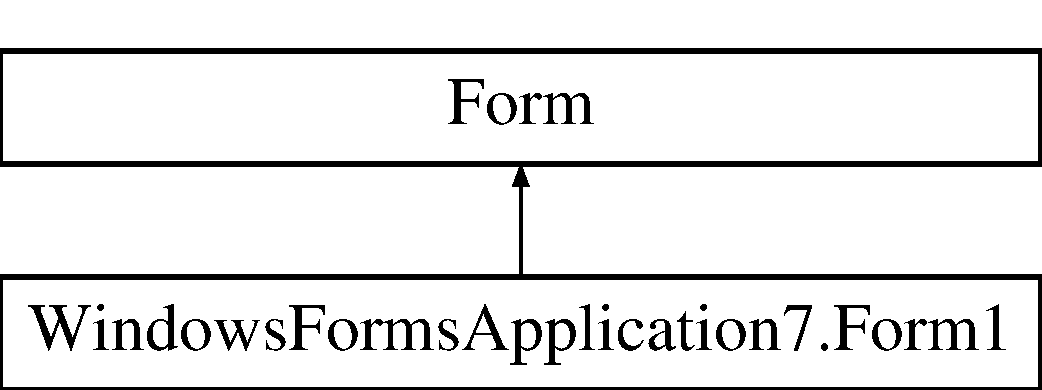
\includegraphics[height=2.000000cm]{class_windows_forms_application7_1_1_form1}
\end{center}
\end{figure}
\subsection*{Chráněné metody}
\begin{DoxyCompactItemize}
\item 
override void \hyperlink{class_windows_forms_application7_1_1_form1_a8a3de7949c73c2d190c437c57d1a514a}{Dispose} (bool disposing)
\begin{DoxyCompactList}\small\item\em Clean up any resources being used. \end{DoxyCompactList}\end{DoxyCompactItemize}
\subsection*{Privátní metody}
\begin{DoxyCompactItemize}
\item 
void \hyperlink{class_windows_forms_application7_1_1_form1_a3d30a8143ce023ef6241f6e3b9f0a933}{button1\+\_\+\+Click} (object sender, Event\+Args e)
\begin{DoxyCompactList}\small\item\em Metoda vyčistí text\+Box a zajistí aby byla zadána nejvýše jedna desetinná čárka. \end{DoxyCompactList}\item 
void \hyperlink{class_windows_forms_application7_1_1_form1_ad911bf5bdbec7c25585694c4c1520cd6}{button17\+\_\+\+Click} (object sender, Event\+Args e)
\begin{DoxyCompactList}\small\item\em Metoda nastaví počáteční příznaky jednotlivých operací na default. \end{DoxyCompactList}\item 
void \hyperlink{class_windows_forms_application7_1_1_form1_a4f79ca83e4dc1e9bcd343a5cb3a86273}{button11\+\_\+\+Click} (object sender, Event\+Args e)
\begin{DoxyCompactList}\small\item\em Metoda zabrání v zadání více znamének operace za sebou, nastaví příznak operace sčítání na true, načte první číslo pro sčítání a zobrazí jej spolu se znakem \textquotesingle{}+\textquotesingle{} do labelu. \end{DoxyCompactList}\item 
void \hyperlink{class_windows_forms_application7_1_1_form1_ad550bcffb060db5fbddc045e6a0e81f7}{button12\+\_\+\+Click} (object sender, Event\+Args e)
\begin{DoxyCompactList}\small\item\em Metoda zabrání v zadání více znamének operace za sebou, nastaví příznak operace odečítání na true, načte první číslo pro tuto operaci a zobrazí jej spolu se znakem \textquotesingle{}-\/\textquotesingle{} do labelu. \end{DoxyCompactList}\item 
void \hyperlink{class_windows_forms_application7_1_1_form1_a70b0c4d24d34b89e6b1303d95fb0617f}{button13\+\_\+\+Click} (object sender, Event\+Args e)
\begin{DoxyCompactList}\small\item\em Metoda zabrání v zadání více znamének operace za sebou, nastaví příznak operace násobení na true, načte první číslo pro tuto operaci a zobrazí jej spolu se znakem \textquotesingle{}$\ast$\textquotesingle{} do labelu. \end{DoxyCompactList}\item 
void \hyperlink{class_windows_forms_application7_1_1_form1_a8adbbb58ffa0e57bbc3a15ecbd0cbabf}{button14\+\_\+\+Click} (object sender, Event\+Args e)
\begin{DoxyCompactList}\small\item\em Metoda zabrání v zadání více znamének operace za sebou, nastaví příznak operace dělení na true, načte první číslo pro tuto operaci a zobrazí jej spolu se znakem \textquotesingle{}/\textquotesingle{} do labelu. \end{DoxyCompactList}\item 
void \hyperlink{class_windows_forms_application7_1_1_form1_a0932cba64dc5f9adad5071abcb250ab6}{button15\+\_\+\+Click} (object sender, Event\+Args e)
\begin{DoxyCompactList}\small\item\em Metoda načte druhé číslo dané operace s nastaveným příznakem na true, vypíše jej spolu se znakem \textquotesingle{}=\textquotesingle{} do labelu a do text\+Boxu zobrazí výsledek dané operace. Nakonec nastaví příznak dané operace na false. \end{DoxyCompactList}\item 
void \hyperlink{class_windows_forms_application7_1_1_form1_a32b4400be4c04cf62eb1a9212ca741ae}{button18\+\_\+\+Click} (object sender, Event\+Args e)
\begin{DoxyCompactList}\small\item\em Metoda zabrání v zadání více znamének operace za sebou, nastaví příznak operace faktoriál na true Načte číslo pro tuto operaci, zobrazí jej spolu se znakem \textquotesingle{}!\textquotesingle{} do labelu a výsledek vypíše do text\+Boxu. \end{DoxyCompactList}\item 
void \hyperlink{class_windows_forms_application7_1_1_form1_ae9109c88bfb8ffd8232e2ca811ac0aad}{button19\+\_\+\+Click} (object sender, Event\+Args e)
\begin{DoxyCompactList}\small\item\em Metoda zabrání v zadání více znamének operace za sebou, nastaví příznak operace mocnina (pow) na true, načte číslo (základ) pro tuto operaci a zobrazí jej spolu se znakem \textquotesingle{}$^\wedge$\textquotesingle{} do labelu. \end{DoxyCompactList}\item 
void \hyperlink{class_windows_forms_application7_1_1_form1_aaf84d0ede48547de6a9a4a0b454c5523}{button20\+\_\+\+Click} (object sender, Event\+Args e)
\begin{DoxyCompactList}\small\item\em Metoda zabrání v zadání více znamének operace za sebou, nastaví příznak operace modulo (zbytej po celočíselném dělení) na true, načte první číslo pro tuto operaci a zobrazí jej spolu se znakem \textquotesingle{}\textquotesingle{} do labelu. \end{DoxyCompactList}\item 
void \hyperlink{class_windows_forms_application7_1_1_form1_a7d5f405d8a73d3ebf3719bbe353b5347}{button21\+\_\+\+Click} (object sender, Event\+Args e)
\begin{DoxyCompactList}\small\item\em Metoda zabrání v zadání více znamének operace za sebou, nastaví příznak operace odmocniny (sqrt) na true, načte první číslo pro tuto operaci a zobrazí jej spolu se znakem \textquotesingle{}√\textquotesingle{} do labelu. \end{DoxyCompactList}\item 
void \hyperlink{class_windows_forms_application7_1_1_form1_aa43c2856c44afb199010bddbcb20c645}{Exit\+\_\+\+Click} (object sender, Event\+Args e)
\begin{DoxyCompactList}\small\item\em Metoda uzavře aplikaci na deném tlačítku. \end{DoxyCompactList}\item 
void {\bfseries text\+Box1\+\_\+\+Text\+Changed} (object sender, Event\+Args e)\hypertarget{class_windows_forms_application7_1_1_form1_ac5e3c96c35111db5d1784a6f767b3eb4}{}\label{class_windows_forms_application7_1_1_form1_ac5e3c96c35111db5d1784a6f767b3eb4}

\item 
void {\bfseries Form1\+\_\+\+Load} (object sender, Event\+Args e)\hypertarget{class_windows_forms_application7_1_1_form1_ab5a9a2061ddb51fd956ae7a6e4e36017}{}\label{class_windows_forms_application7_1_1_form1_ab5a9a2061ddb51fd956ae7a6e4e36017}

\item 
void {\bfseries Form1\+\_\+\+Mouse\+Down} (object sender, Mouse\+Event\+Args e)\hypertarget{class_windows_forms_application7_1_1_form1_a0a831adb1b6d4ec3739a66592d83b6a8}{}\label{class_windows_forms_application7_1_1_form1_a0a831adb1b6d4ec3739a66592d83b6a8}

\item 
void \hyperlink{class_windows_forms_application7_1_1_form1_a9cc4356fccd25fe5fa780e9eb0a540cf}{Initialize\+Component} ()
\begin{DoxyCompactList}\small\item\em Required method for Designer support -\/ do not modify the contents of this method with the code editor. \end{DoxyCompactList}\end{DoxyCompactItemize}
\subsection*{Privátní atributy}
\begin{DoxyCompactItemize}
\item 
Boolean {\bfseries test\+\_\+comma} = false\hypertarget{class_windows_forms_application7_1_1_form1_a1e1b4c6fdaceb744c49b9a2b60b77a4c}{}\label{class_windows_forms_application7_1_1_form1_a1e1b4c6fdaceb744c49b9a2b60b77a4c}

\item 
Boolean {\bfseries operace\+\_\+scitani} = false\hypertarget{class_windows_forms_application7_1_1_form1_a3991c59c9a6072db35eac89d37b70d67}{}\label{class_windows_forms_application7_1_1_form1_a3991c59c9a6072db35eac89d37b70d67}

\item 
Boolean {\bfseries operace\+\_\+odcitani} = false\hypertarget{class_windows_forms_application7_1_1_form1_a11d770af092cbf3d0ba01cf0b0094cf7}{}\label{class_windows_forms_application7_1_1_form1_a11d770af092cbf3d0ba01cf0b0094cf7}

\item 
Boolean {\bfseries operace\+\_\+nasobeni} = false\hypertarget{class_windows_forms_application7_1_1_form1_af73e8271ded3255a8f636697b7361d0a}{}\label{class_windows_forms_application7_1_1_form1_af73e8271ded3255a8f636697b7361d0a}

\item 
Boolean {\bfseries operace\+\_\+deleni} = false\hypertarget{class_windows_forms_application7_1_1_form1_a8eee77affc99503ee52951c187e9deaf}{}\label{class_windows_forms_application7_1_1_form1_a8eee77affc99503ee52951c187e9deaf}

\item 
Boolean {\bfseries operace\+\_\+faktorial} = false\hypertarget{class_windows_forms_application7_1_1_form1_a0dc8f91f53cdd887777eed0d32697db8}{}\label{class_windows_forms_application7_1_1_form1_a0dc8f91f53cdd887777eed0d32697db8}

\item 
Boolean {\bfseries operace\+\_\+pow} = false\hypertarget{class_windows_forms_application7_1_1_form1_ad055159307cd27ccbb40bc4744702658}{}\label{class_windows_forms_application7_1_1_form1_ad055159307cd27ccbb40bc4744702658}

\item 
Boolean {\bfseries zvysok\+\_\+del} = false\hypertarget{class_windows_forms_application7_1_1_form1_a96971b16821c8587f23ab4dd993f5669}{}\label{class_windows_forms_application7_1_1_form1_a96971b16821c8587f23ab4dd993f5669}

\item 
Boolean {\bfseries operace\+\_\+sqrt} = false\hypertarget{class_windows_forms_application7_1_1_form1_a8bd9e8ef249f029fa40e57aa3174a503}{}\label{class_windows_forms_application7_1_1_form1_a8bd9e8ef249f029fa40e57aa3174a503}

\item 
double {\bfseries operand1} = 0\hypertarget{class_windows_forms_application7_1_1_form1_aec9aee3dc421f608d443d33495559958}{}\label{class_windows_forms_application7_1_1_form1_aec9aee3dc421f608d443d33495559958}

\item 
double {\bfseries operand2} = 0\hypertarget{class_windows_forms_application7_1_1_form1_ac1a57710bb57f32de2414de515173528}{}\label{class_windows_forms_application7_1_1_form1_ac1a57710bb57f32de2414de515173528}

\item 
double {\bfseries vysledok} = 0\hypertarget{class_windows_forms_application7_1_1_form1_a8c29e2f179d06ce59b1544d133533d1e}{}\label{class_windows_forms_application7_1_1_form1_a8c29e2f179d06ce59b1544d133533d1e}

\item 
matematicka.\+Class1 {\bfseries new\+Object} = new matematicka.\+Class1()\hypertarget{class_windows_forms_application7_1_1_form1_ab464987fdce1f221be67c20ceb8b9e94}{}\label{class_windows_forms_application7_1_1_form1_ab464987fdce1f221be67c20ceb8b9e94}

\item 
System.\+Component\+Model.\+I\+Container \hyperlink{class_windows_forms_application7_1_1_form1_a40a2aa9887f212867bdfee9a667b9860}{components} = null
\begin{DoxyCompactList}\small\item\em Required designer variable. \end{DoxyCompactList}\item 
System.\+Windows.\+Forms.\+Text\+Box {\bfseries text\+Box1}\hypertarget{class_windows_forms_application7_1_1_form1_a812b1e343c0c28b14687bbcff0abf524}{}\label{class_windows_forms_application7_1_1_form1_a812b1e343c0c28b14687bbcff0abf524}

\item 
System.\+Windows.\+Forms.\+Button {\bfseries button1}\hypertarget{class_windows_forms_application7_1_1_form1_aad417f0c4fb3c2a3dfcd1a25396aee9e}{}\label{class_windows_forms_application7_1_1_form1_aad417f0c4fb3c2a3dfcd1a25396aee9e}

\item 
System.\+Windows.\+Forms.\+Button {\bfseries button2}\hypertarget{class_windows_forms_application7_1_1_form1_ae79069e1e69955d1312c544bc0556bd3}{}\label{class_windows_forms_application7_1_1_form1_ae79069e1e69955d1312c544bc0556bd3}

\item 
System.\+Windows.\+Forms.\+Button {\bfseries button3}\hypertarget{class_windows_forms_application7_1_1_form1_a3a748e562cbc619e76384eb3236297a3}{}\label{class_windows_forms_application7_1_1_form1_a3a748e562cbc619e76384eb3236297a3}

\item 
System.\+Windows.\+Forms.\+Button {\bfseries button4}\hypertarget{class_windows_forms_application7_1_1_form1_af50e03a38d7997104bbbc1d8955772b7}{}\label{class_windows_forms_application7_1_1_form1_af50e03a38d7997104bbbc1d8955772b7}

\item 
System.\+Windows.\+Forms.\+Button {\bfseries button5}\hypertarget{class_windows_forms_application7_1_1_form1_a9fa591f3cb9af34b0a45da212ef71621}{}\label{class_windows_forms_application7_1_1_form1_a9fa591f3cb9af34b0a45da212ef71621}

\item 
System.\+Windows.\+Forms.\+Button {\bfseries button6}\hypertarget{class_windows_forms_application7_1_1_form1_a70ba51f085e89b6d4fe7d5ef752ea79a}{}\label{class_windows_forms_application7_1_1_form1_a70ba51f085e89b6d4fe7d5ef752ea79a}

\item 
System.\+Windows.\+Forms.\+Button {\bfseries button7}\hypertarget{class_windows_forms_application7_1_1_form1_a781817e035085916558bb204a9d68466}{}\label{class_windows_forms_application7_1_1_form1_a781817e035085916558bb204a9d68466}

\item 
System.\+Windows.\+Forms.\+Button {\bfseries button8}\hypertarget{class_windows_forms_application7_1_1_form1_a04e36d02faec3c9d9224a89924f9081a}{}\label{class_windows_forms_application7_1_1_form1_a04e36d02faec3c9d9224a89924f9081a}

\item 
System.\+Windows.\+Forms.\+Button {\bfseries button9}\hypertarget{class_windows_forms_application7_1_1_form1_a6f09d0033f04c5b618a89dae214e7705}{}\label{class_windows_forms_application7_1_1_form1_a6f09d0033f04c5b618a89dae214e7705}

\item 
System.\+Windows.\+Forms.\+Button {\bfseries button10}\hypertarget{class_windows_forms_application7_1_1_form1_afcc21dd721ecc1a719e81a8cb4232dad}{}\label{class_windows_forms_application7_1_1_form1_afcc21dd721ecc1a719e81a8cb4232dad}

\item 
System.\+Windows.\+Forms.\+Button {\bfseries button11}\hypertarget{class_windows_forms_application7_1_1_form1_abbd76841cc9f22230e4326c16739e274}{}\label{class_windows_forms_application7_1_1_form1_abbd76841cc9f22230e4326c16739e274}

\item 
System.\+Windows.\+Forms.\+Button {\bfseries button12}\hypertarget{class_windows_forms_application7_1_1_form1_a837954a532f3c5ef2e3d6fef311e6a0c}{}\label{class_windows_forms_application7_1_1_form1_a837954a532f3c5ef2e3d6fef311e6a0c}

\item 
System.\+Windows.\+Forms.\+Button {\bfseries button13}\hypertarget{class_windows_forms_application7_1_1_form1_a55d666342c53c00819502dcce0cbb9c3}{}\label{class_windows_forms_application7_1_1_form1_a55d666342c53c00819502dcce0cbb9c3}

\item 
System.\+Windows.\+Forms.\+Button {\bfseries button14}\hypertarget{class_windows_forms_application7_1_1_form1_a8396ce75e31cd7f7f8b3577e51d7aa3c}{}\label{class_windows_forms_application7_1_1_form1_a8396ce75e31cd7f7f8b3577e51d7aa3c}

\item 
System.\+Windows.\+Forms.\+Button {\bfseries button15}\hypertarget{class_windows_forms_application7_1_1_form1_a4407e39f2b8f79cd9cf7739a8f47451e}{}\label{class_windows_forms_application7_1_1_form1_a4407e39f2b8f79cd9cf7739a8f47451e}

\item 
System.\+Windows.\+Forms.\+Button {\bfseries button16}\hypertarget{class_windows_forms_application7_1_1_form1_a661b60260d1ff7950742527170aa6e01}{}\label{class_windows_forms_application7_1_1_form1_a661b60260d1ff7950742527170aa6e01}

\item 
System.\+Windows.\+Forms.\+Button {\bfseries button17}\hypertarget{class_windows_forms_application7_1_1_form1_a4ab6a38717631871f27a245512bf5b79}{}\label{class_windows_forms_application7_1_1_form1_a4ab6a38717631871f27a245512bf5b79}

\item 
System.\+Windows.\+Forms.\+Label {\bfseries label1}\hypertarget{class_windows_forms_application7_1_1_form1_ac92c3f1e1f97188e68f156790f69c167}{}\label{class_windows_forms_application7_1_1_form1_ac92c3f1e1f97188e68f156790f69c167}

\item 
System.\+Windows.\+Forms.\+Button {\bfseries button18}\hypertarget{class_windows_forms_application7_1_1_form1_a40289766f48462543094b9b5dbab4dba}{}\label{class_windows_forms_application7_1_1_form1_a40289766f48462543094b9b5dbab4dba}

\item 
System.\+Windows.\+Forms.\+Button {\bfseries button19}\hypertarget{class_windows_forms_application7_1_1_form1_a48aa1bae0e06cd8aae7cc28e0a94a9b6}{}\label{class_windows_forms_application7_1_1_form1_a48aa1bae0e06cd8aae7cc28e0a94a9b6}

\item 
System.\+Windows.\+Forms.\+Button {\bfseries button20}\hypertarget{class_windows_forms_application7_1_1_form1_a5728919bf8c392d6f072ad31b374a7ea}{}\label{class_windows_forms_application7_1_1_form1_a5728919bf8c392d6f072ad31b374a7ea}

\item 
System.\+Windows.\+Forms.\+Button {\bfseries button21}\hypertarget{class_windows_forms_application7_1_1_form1_a7b774c29d8ea3266a5d9a532a181a451}{}\label{class_windows_forms_application7_1_1_form1_a7b774c29d8ea3266a5d9a532a181a451}

\item 
System.\+Windows.\+Forms.\+Button {\bfseries Exit}\hypertarget{class_windows_forms_application7_1_1_form1_af58a108a88858ea6b7fa37c7167315b7}{}\label{class_windows_forms_application7_1_1_form1_af58a108a88858ea6b7fa37c7167315b7}

\item 
System.\+Windows.\+Forms.\+Button {\bfseries Minimalize}\hypertarget{class_windows_forms_application7_1_1_form1_a8966c3b203972856ad144621e1204fd7}{}\label{class_windows_forms_application7_1_1_form1_a8966c3b203972856ad144621e1204fd7}

\end{DoxyCompactItemize}


\subsection{Dokumentace k metodám}
\index{Windows\+Forms\+Application7\+::\+Form1@{Windows\+Forms\+Application7\+::\+Form1}!button11\+\_\+\+Click@{button11\+\_\+\+Click}}
\index{button11\+\_\+\+Click@{button11\+\_\+\+Click}!Windows\+Forms\+Application7\+::\+Form1@{Windows\+Forms\+Application7\+::\+Form1}}
\subsubsection[{\texorpdfstring{button11\+\_\+\+Click(object sender, Event\+Args e)}{button11_Click(object sender, EventArgs e)}}]{\setlength{\rightskip}{0pt plus 5cm}void Windows\+Forms\+Application7.\+Form1.\+button11\+\_\+\+Click (
\begin{DoxyParamCaption}
\item[{object}]{sender, }
\item[{Event\+Args}]{e}
\end{DoxyParamCaption}
)\hspace{0.3cm}{\ttfamily [private]}}\hypertarget{class_windows_forms_application7_1_1_form1_a4f79ca83e4dc1e9bcd343a5cb3a86273}{}\label{class_windows_forms_application7_1_1_form1_a4f79ca83e4dc1e9bcd343a5cb3a86273}


Metoda zabrání v zadání více znamének operace za sebou, nastaví příznak operace sčítání na true, načte první číslo pro sčítání a zobrazí jej spolu se znakem \textquotesingle{}+\textquotesingle{} do labelu. 

\index{Windows\+Forms\+Application7\+::\+Form1@{Windows\+Forms\+Application7\+::\+Form1}!button12\+\_\+\+Click@{button12\+\_\+\+Click}}
\index{button12\+\_\+\+Click@{button12\+\_\+\+Click}!Windows\+Forms\+Application7\+::\+Form1@{Windows\+Forms\+Application7\+::\+Form1}}
\subsubsection[{\texorpdfstring{button12\+\_\+\+Click(object sender, Event\+Args e)}{button12_Click(object sender, EventArgs e)}}]{\setlength{\rightskip}{0pt plus 5cm}void Windows\+Forms\+Application7.\+Form1.\+button12\+\_\+\+Click (
\begin{DoxyParamCaption}
\item[{object}]{sender, }
\item[{Event\+Args}]{e}
\end{DoxyParamCaption}
)\hspace{0.3cm}{\ttfamily [private]}}\hypertarget{class_windows_forms_application7_1_1_form1_ad550bcffb060db5fbddc045e6a0e81f7}{}\label{class_windows_forms_application7_1_1_form1_ad550bcffb060db5fbddc045e6a0e81f7}


Metoda zabrání v zadání více znamének operace za sebou, nastaví příznak operace odečítání na true, načte první číslo pro tuto operaci a zobrazí jej spolu se znakem \textquotesingle{}-\/\textquotesingle{} do labelu. 

\index{Windows\+Forms\+Application7\+::\+Form1@{Windows\+Forms\+Application7\+::\+Form1}!button13\+\_\+\+Click@{button13\+\_\+\+Click}}
\index{button13\+\_\+\+Click@{button13\+\_\+\+Click}!Windows\+Forms\+Application7\+::\+Form1@{Windows\+Forms\+Application7\+::\+Form1}}
\subsubsection[{\texorpdfstring{button13\+\_\+\+Click(object sender, Event\+Args e)}{button13_Click(object sender, EventArgs e)}}]{\setlength{\rightskip}{0pt plus 5cm}void Windows\+Forms\+Application7.\+Form1.\+button13\+\_\+\+Click (
\begin{DoxyParamCaption}
\item[{object}]{sender, }
\item[{Event\+Args}]{e}
\end{DoxyParamCaption}
)\hspace{0.3cm}{\ttfamily [private]}}\hypertarget{class_windows_forms_application7_1_1_form1_a70b0c4d24d34b89e6b1303d95fb0617f}{}\label{class_windows_forms_application7_1_1_form1_a70b0c4d24d34b89e6b1303d95fb0617f}


Metoda zabrání v zadání více znamének operace za sebou, nastaví příznak operace násobení na true, načte první číslo pro tuto operaci a zobrazí jej spolu se znakem \textquotesingle{}$\ast$\textquotesingle{} do labelu. 


\begin{DoxyParams}{Parametry}
{\em sender} & \\
\hline
{\em e} & \\
\hline
\end{DoxyParams}
\index{Windows\+Forms\+Application7\+::\+Form1@{Windows\+Forms\+Application7\+::\+Form1}!button14\+\_\+\+Click@{button14\+\_\+\+Click}}
\index{button14\+\_\+\+Click@{button14\+\_\+\+Click}!Windows\+Forms\+Application7\+::\+Form1@{Windows\+Forms\+Application7\+::\+Form1}}
\subsubsection[{\texorpdfstring{button14\+\_\+\+Click(object sender, Event\+Args e)}{button14_Click(object sender, EventArgs e)}}]{\setlength{\rightskip}{0pt plus 5cm}void Windows\+Forms\+Application7.\+Form1.\+button14\+\_\+\+Click (
\begin{DoxyParamCaption}
\item[{object}]{sender, }
\item[{Event\+Args}]{e}
\end{DoxyParamCaption}
)\hspace{0.3cm}{\ttfamily [private]}}\hypertarget{class_windows_forms_application7_1_1_form1_a8adbbb58ffa0e57bbc3a15ecbd0cbabf}{}\label{class_windows_forms_application7_1_1_form1_a8adbbb58ffa0e57bbc3a15ecbd0cbabf}


Metoda zabrání v zadání více znamének operace za sebou, nastaví příznak operace dělení na true, načte první číslo pro tuto operaci a zobrazí jej spolu se znakem \textquotesingle{}/\textquotesingle{} do labelu. 

\index{Windows\+Forms\+Application7\+::\+Form1@{Windows\+Forms\+Application7\+::\+Form1}!button15\+\_\+\+Click@{button15\+\_\+\+Click}}
\index{button15\+\_\+\+Click@{button15\+\_\+\+Click}!Windows\+Forms\+Application7\+::\+Form1@{Windows\+Forms\+Application7\+::\+Form1}}
\subsubsection[{\texorpdfstring{button15\+\_\+\+Click(object sender, Event\+Args e)}{button15_Click(object sender, EventArgs e)}}]{\setlength{\rightskip}{0pt plus 5cm}void Windows\+Forms\+Application7.\+Form1.\+button15\+\_\+\+Click (
\begin{DoxyParamCaption}
\item[{object}]{sender, }
\item[{Event\+Args}]{e}
\end{DoxyParamCaption}
)\hspace{0.3cm}{\ttfamily [private]}}\hypertarget{class_windows_forms_application7_1_1_form1_a0932cba64dc5f9adad5071abcb250ab6}{}\label{class_windows_forms_application7_1_1_form1_a0932cba64dc5f9adad5071abcb250ab6}


Metoda načte druhé číslo dané operace s nastaveným příznakem na true, vypíše jej spolu se znakem \textquotesingle{}=\textquotesingle{} do labelu a do text\+Boxu zobrazí výsledek dané operace. Nakonec nastaví příznak dané operace na false. 

\index{Windows\+Forms\+Application7\+::\+Form1@{Windows\+Forms\+Application7\+::\+Form1}!button17\+\_\+\+Click@{button17\+\_\+\+Click}}
\index{button17\+\_\+\+Click@{button17\+\_\+\+Click}!Windows\+Forms\+Application7\+::\+Form1@{Windows\+Forms\+Application7\+::\+Form1}}
\subsubsection[{\texorpdfstring{button17\+\_\+\+Click(object sender, Event\+Args e)}{button17_Click(object sender, EventArgs e)}}]{\setlength{\rightskip}{0pt plus 5cm}void Windows\+Forms\+Application7.\+Form1.\+button17\+\_\+\+Click (
\begin{DoxyParamCaption}
\item[{object}]{sender, }
\item[{Event\+Args}]{e}
\end{DoxyParamCaption}
)\hspace{0.3cm}{\ttfamily [private]}}\hypertarget{class_windows_forms_application7_1_1_form1_ad911bf5bdbec7c25585694c4c1520cd6}{}\label{class_windows_forms_application7_1_1_form1_ad911bf5bdbec7c25585694c4c1520cd6}


Metoda nastaví počáteční příznaky jednotlivých operací na default. 

\index{Windows\+Forms\+Application7\+::\+Form1@{Windows\+Forms\+Application7\+::\+Form1}!button18\+\_\+\+Click@{button18\+\_\+\+Click}}
\index{button18\+\_\+\+Click@{button18\+\_\+\+Click}!Windows\+Forms\+Application7\+::\+Form1@{Windows\+Forms\+Application7\+::\+Form1}}
\subsubsection[{\texorpdfstring{button18\+\_\+\+Click(object sender, Event\+Args e)}{button18_Click(object sender, EventArgs e)}}]{\setlength{\rightskip}{0pt plus 5cm}void Windows\+Forms\+Application7.\+Form1.\+button18\+\_\+\+Click (
\begin{DoxyParamCaption}
\item[{object}]{sender, }
\item[{Event\+Args}]{e}
\end{DoxyParamCaption}
)\hspace{0.3cm}{\ttfamily [private]}}\hypertarget{class_windows_forms_application7_1_1_form1_a32b4400be4c04cf62eb1a9212ca741ae}{}\label{class_windows_forms_application7_1_1_form1_a32b4400be4c04cf62eb1a9212ca741ae}


Metoda zabrání v zadání více znamének operace za sebou, nastaví příznak operace faktoriál na true Načte číslo pro tuto operaci, zobrazí jej spolu se znakem \textquotesingle{}!\textquotesingle{} do labelu a výsledek vypíše do text\+Boxu. 

\index{Windows\+Forms\+Application7\+::\+Form1@{Windows\+Forms\+Application7\+::\+Form1}!button19\+\_\+\+Click@{button19\+\_\+\+Click}}
\index{button19\+\_\+\+Click@{button19\+\_\+\+Click}!Windows\+Forms\+Application7\+::\+Form1@{Windows\+Forms\+Application7\+::\+Form1}}
\subsubsection[{\texorpdfstring{button19\+\_\+\+Click(object sender, Event\+Args e)}{button19_Click(object sender, EventArgs e)}}]{\setlength{\rightskip}{0pt plus 5cm}void Windows\+Forms\+Application7.\+Form1.\+button19\+\_\+\+Click (
\begin{DoxyParamCaption}
\item[{object}]{sender, }
\item[{Event\+Args}]{e}
\end{DoxyParamCaption}
)\hspace{0.3cm}{\ttfamily [private]}}\hypertarget{class_windows_forms_application7_1_1_form1_ae9109c88bfb8ffd8232e2ca811ac0aad}{}\label{class_windows_forms_application7_1_1_form1_ae9109c88bfb8ffd8232e2ca811ac0aad}


Metoda zabrání v zadání více znamének operace za sebou, nastaví příznak operace mocnina (pow) na true, načte číslo (základ) pro tuto operaci a zobrazí jej spolu se znakem \textquotesingle{}$^\wedge$\textquotesingle{} do labelu. 


\begin{DoxyParams}{Parametry}
{\em sender} & \\
\hline
\end{DoxyParams}
\index{Windows\+Forms\+Application7\+::\+Form1@{Windows\+Forms\+Application7\+::\+Form1}!button1\+\_\+\+Click@{button1\+\_\+\+Click}}
\index{button1\+\_\+\+Click@{button1\+\_\+\+Click}!Windows\+Forms\+Application7\+::\+Form1@{Windows\+Forms\+Application7\+::\+Form1}}
\subsubsection[{\texorpdfstring{button1\+\_\+\+Click(object sender, Event\+Args e)}{button1_Click(object sender, EventArgs e)}}]{\setlength{\rightskip}{0pt plus 5cm}void Windows\+Forms\+Application7.\+Form1.\+button1\+\_\+\+Click (
\begin{DoxyParamCaption}
\item[{object}]{sender, }
\item[{Event\+Args}]{e}
\end{DoxyParamCaption}
)\hspace{0.3cm}{\ttfamily [private]}}\hypertarget{class_windows_forms_application7_1_1_form1_a3d30a8143ce023ef6241f6e3b9f0a933}{}\label{class_windows_forms_application7_1_1_form1_a3d30a8143ce023ef6241f6e3b9f0a933}


Metoda vyčistí text\+Box a zajistí aby byla zadána nejvýše jedna desetinná čárka. 

\index{Windows\+Forms\+Application7\+::\+Form1@{Windows\+Forms\+Application7\+::\+Form1}!button20\+\_\+\+Click@{button20\+\_\+\+Click}}
\index{button20\+\_\+\+Click@{button20\+\_\+\+Click}!Windows\+Forms\+Application7\+::\+Form1@{Windows\+Forms\+Application7\+::\+Form1}}
\subsubsection[{\texorpdfstring{button20\+\_\+\+Click(object sender, Event\+Args e)}{button20_Click(object sender, EventArgs e)}}]{\setlength{\rightskip}{0pt plus 5cm}void Windows\+Forms\+Application7.\+Form1.\+button20\+\_\+\+Click (
\begin{DoxyParamCaption}
\item[{object}]{sender, }
\item[{Event\+Args}]{e}
\end{DoxyParamCaption}
)\hspace{0.3cm}{\ttfamily [private]}}\hypertarget{class_windows_forms_application7_1_1_form1_aaf84d0ede48547de6a9a4a0b454c5523}{}\label{class_windows_forms_application7_1_1_form1_aaf84d0ede48547de6a9a4a0b454c5523}


Metoda zabrání v zadání více znamének operace za sebou, nastaví příznak operace modulo (zbytej po celočíselném dělení) na true, načte první číslo pro tuto operaci a zobrazí jej spolu se znakem \textquotesingle{}\textquotesingle{} do labelu. 

\index{Windows\+Forms\+Application7\+::\+Form1@{Windows\+Forms\+Application7\+::\+Form1}!button21\+\_\+\+Click@{button21\+\_\+\+Click}}
\index{button21\+\_\+\+Click@{button21\+\_\+\+Click}!Windows\+Forms\+Application7\+::\+Form1@{Windows\+Forms\+Application7\+::\+Form1}}
\subsubsection[{\texorpdfstring{button21\+\_\+\+Click(object sender, Event\+Args e)}{button21_Click(object sender, EventArgs e)}}]{\setlength{\rightskip}{0pt plus 5cm}void Windows\+Forms\+Application7.\+Form1.\+button21\+\_\+\+Click (
\begin{DoxyParamCaption}
\item[{object}]{sender, }
\item[{Event\+Args}]{e}
\end{DoxyParamCaption}
)\hspace{0.3cm}{\ttfamily [private]}}\hypertarget{class_windows_forms_application7_1_1_form1_a7d5f405d8a73d3ebf3719bbe353b5347}{}\label{class_windows_forms_application7_1_1_form1_a7d5f405d8a73d3ebf3719bbe353b5347}


Metoda zabrání v zadání více znamének operace za sebou, nastaví příznak operace odmocniny (sqrt) na true, načte první číslo pro tuto operaci a zobrazí jej spolu se znakem \textquotesingle{}√\textquotesingle{} do labelu. 

\index{Windows\+Forms\+Application7\+::\+Form1@{Windows\+Forms\+Application7\+::\+Form1}!Dispose@{Dispose}}
\index{Dispose@{Dispose}!Windows\+Forms\+Application7\+::\+Form1@{Windows\+Forms\+Application7\+::\+Form1}}
\subsubsection[{\texorpdfstring{Dispose(bool disposing)}{Dispose(bool disposing)}}]{\setlength{\rightskip}{0pt plus 5cm}override void Windows\+Forms\+Application7.\+Form1.\+Dispose (
\begin{DoxyParamCaption}
\item[{bool}]{disposing}
\end{DoxyParamCaption}
)\hspace{0.3cm}{\ttfamily [protected]}}\hypertarget{class_windows_forms_application7_1_1_form1_a8a3de7949c73c2d190c437c57d1a514a}{}\label{class_windows_forms_application7_1_1_form1_a8a3de7949c73c2d190c437c57d1a514a}


Clean up any resources being used. 


\begin{DoxyParams}{Parametry}
{\em disposing} & true if managed resources should be disposed; otherwise, false.\\
\hline
\end{DoxyParams}
\index{Windows\+Forms\+Application7\+::\+Form1@{Windows\+Forms\+Application7\+::\+Form1}!Exit\+\_\+\+Click@{Exit\+\_\+\+Click}}
\index{Exit\+\_\+\+Click@{Exit\+\_\+\+Click}!Windows\+Forms\+Application7\+::\+Form1@{Windows\+Forms\+Application7\+::\+Form1}}
\subsubsection[{\texorpdfstring{Exit\+\_\+\+Click(object sender, Event\+Args e)}{Exit_Click(object sender, EventArgs e)}}]{\setlength{\rightskip}{0pt plus 5cm}void Windows\+Forms\+Application7.\+Form1.\+Exit\+\_\+\+Click (
\begin{DoxyParamCaption}
\item[{object}]{sender, }
\item[{Event\+Args}]{e}
\end{DoxyParamCaption}
)\hspace{0.3cm}{\ttfamily [private]}}\hypertarget{class_windows_forms_application7_1_1_form1_aa43c2856c44afb199010bddbcb20c645}{}\label{class_windows_forms_application7_1_1_form1_aa43c2856c44afb199010bddbcb20c645}


Metoda uzavře aplikaci na deném tlačítku. 

\index{Windows\+Forms\+Application7\+::\+Form1@{Windows\+Forms\+Application7\+::\+Form1}!Initialize\+Component@{Initialize\+Component}}
\index{Initialize\+Component@{Initialize\+Component}!Windows\+Forms\+Application7\+::\+Form1@{Windows\+Forms\+Application7\+::\+Form1}}
\subsubsection[{\texorpdfstring{Initialize\+Component()}{InitializeComponent()}}]{\setlength{\rightskip}{0pt plus 5cm}void Windows\+Forms\+Application7.\+Form1.\+Initialize\+Component (
\begin{DoxyParamCaption}
{}
\end{DoxyParamCaption}
)\hspace{0.3cm}{\ttfamily [private]}}\hypertarget{class_windows_forms_application7_1_1_form1_a9cc4356fccd25fe5fa780e9eb0a540cf}{}\label{class_windows_forms_application7_1_1_form1_a9cc4356fccd25fe5fa780e9eb0a540cf}


Required method for Designer support -\/ do not modify the contents of this method with the code editor. 



\subsection{Dokumentace k datovým členům}
\index{Windows\+Forms\+Application7\+::\+Form1@{Windows\+Forms\+Application7\+::\+Form1}!components@{components}}
\index{components@{components}!Windows\+Forms\+Application7\+::\+Form1@{Windows\+Forms\+Application7\+::\+Form1}}
\subsubsection[{\texorpdfstring{components}{components}}]{\setlength{\rightskip}{0pt plus 5cm}System.\+Component\+Model.\+I\+Container Windows\+Forms\+Application7.\+Form1.\+components = null\hspace{0.3cm}{\ttfamily [private]}}\hypertarget{class_windows_forms_application7_1_1_form1_a40a2aa9887f212867bdfee9a667b9860}{}\label{class_windows_forms_application7_1_1_form1_a40a2aa9887f212867bdfee9a667b9860}


Required designer variable. 



Dokumentace pro tuto třídu byla generována z následujících souborů\+:\begin{DoxyCompactItemize}
\item 
C\+:/\+Users/\+Katerina/\+Documents/\+\_\+\+F\+I\+T\+\_\+/\+I\+V\+S/proj2/kalkulacka/\+Windows\+Forms\+Application7/\+Windows\+Forms\+Application7/Form1.\+cs\item 
C\+:/\+Users/\+Katerina/\+Documents/\+\_\+\+F\+I\+T\+\_\+/\+I\+V\+S/proj2/kalkulacka/\+Windows\+Forms\+Application7/\+Windows\+Forms\+Application7/Form1.\+Designer.\+cs\end{DoxyCompactItemize}

\hypertarget{class_windows_forms_application7_1_1_program}{}\section{Dokumentace třídy Windows\+Forms\+Application7.\+Program}
\label{class_windows_forms_application7_1_1_program}\index{Windows\+Forms\+Application7.\+Program@{Windows\+Forms\+Application7.\+Program}}
\subsection*{Statické privátní metody}
\begin{DoxyCompactItemize}
\item 
static void \hyperlink{class_windows_forms_application7_1_1_program_affb16e3d84208c1f0c528a785114a5f9}{Main} ()
\begin{DoxyCompactList}\small\item\em The main entry point for the application. \end{DoxyCompactList}\end{DoxyCompactItemize}


\subsection{Dokumentace k metodám}
\index{Windows\+Forms\+Application7\+::\+Program@{Windows\+Forms\+Application7\+::\+Program}!Main@{Main}}
\index{Main@{Main}!Windows\+Forms\+Application7\+::\+Program@{Windows\+Forms\+Application7\+::\+Program}}
\subsubsection[{\texorpdfstring{Main()}{Main()}}]{\setlength{\rightskip}{0pt plus 5cm}static void Windows\+Forms\+Application7.\+Program.\+Main (
\begin{DoxyParamCaption}
{}
\end{DoxyParamCaption}
)\hspace{0.3cm}{\ttfamily [static]}, {\ttfamily [private]}}\hypertarget{class_windows_forms_application7_1_1_program_affb16e3d84208c1f0c528a785114a5f9}{}\label{class_windows_forms_application7_1_1_program_affb16e3d84208c1f0c528a785114a5f9}


The main entry point for the application. 



Dokumentace pro tuto třídu byla generována z následujícího souboru\+:\begin{DoxyCompactItemize}
\item 
C\+:/\+Users/\+Katerina/\+Documents/\+\_\+\+F\+I\+T\+\_\+/\+I\+V\+S/proj2/kalkulacka/\+Windows\+Forms\+Application7/\+Windows\+Forms\+Application7/Program.\+cs\end{DoxyCompactItemize}

%--- End generated contents ---

% Index
\backmatter
\newpage
\phantomsection
\clearemptydoublepage
\addcontentsline{toc}{chapter}{Rejstřík}
\printindex

\end{document}
